% This LaTeX document needs to be compiled with XeLaTeX.
\documentclass[10pt]{article}
\usepackage[utf8]{inputenc}
\usepackage{amsmath}
\usepackage{amsfonts}
\usepackage{amssymb}
\usepackage[version=4]{mhchem}
\usepackage{stmaryrd}
\usepackage{graphicx}
\usepackage[export]{adjustbox}
\graphicspath{ {./images/} }
\usepackage{multirow}
\usepackage[fallback]{xeCJK}
\usepackage{polyglossia}
\usepackage{fontspec}
\setCJKmainfont{Noto Serif CJK TC}

\setmainlanguage{polish}
\setmainfont{CMU Serif}

\title{Instrukcja dla zdającego }

\author{}
\date{}


\newcommand\Varangle{\mathop{{<\!\!\!\!\!\text{\small)}}\:}\nolimits}

\begin{document}
\maketitle
Czas pracy:

\begin{enumerate}
  \item Sprawdź, czy arkusz zawiera 16 stron.
  \item Rozwiązania zadań i odpowiedzi zamieść w miejscu na to przeznaczonym.
  \item W zadaniach od 1 do 25 są podane 4 odpowiedzi: \(\mathrm{A}, \mathrm{B}, \mathrm{C}, \mathrm{D}\), z których tylko jedna jest prawdziwa. Wybierz tylko jedną odpowiedź i zaznacz ją na karcie odpowiedzi.
  \item Zaznaczając odpowiedzi w części karty przeznaczonej dla zdającego, zamaluj pola do tego przeznaczone. Błędne zaznaczenie otocz kółkiem i zaznacz właściwe.
  \item Rozwiązania zadań od 26 do 34 zapisz starannie i czytelnie w wyznaczonych miejscach. Przedstaw swój tok rozumowania prowadzący do ostatecznego wyniku.
  \item Pamiętaj, że pominięcie argumentacji lub istotnych obliczeń w rozwiązaniu zadania otwartego może spowodować, że za to rozwiązanie możesz nie dostać pełnej liczby punktów.
  \item Pisz czytelnie. Używaj długopisu/pióra tylko z czarnym tuszem/atramentem.
  \item Nie używaj korektora. Błędne zapisy przekreśl.
  \item Pamiętaj, że zapisy w brudnopisie nie podlegają ocenie.
  \item Obok numeru każdego zadania podana jest maksymalna liczba punktów możliwych do uzyskania.
  \item Możesz korzystać z zestawu wzorów matematycznych, cyrkla i linijki oraz kalkulatora.
  \item Wypełnij tę część karty odpowiedzi, którą koduje zdający. Nie wpisuj żadnych znaków części przeznaczonej dla egzaminatora.
\end{enumerate}

Liczba\\
punktów\\
do\\
uzyskania:\\
50

\section*{ZADANIA ZAMKNIETE}
W zadaniach o numerach od 1 do 25 wybierz i zaznacz na karcie odpowiedzi jedną poprawną odpowiedź.

Zadanie 1. (1pkt)\\
Dane są zbiory: \(A=\langle-5 ; 3)\) oraz \(B=\langle 2 ; 7)\). Zbiór \(A \cap B\) zaznaczony jest na rysunku:\\
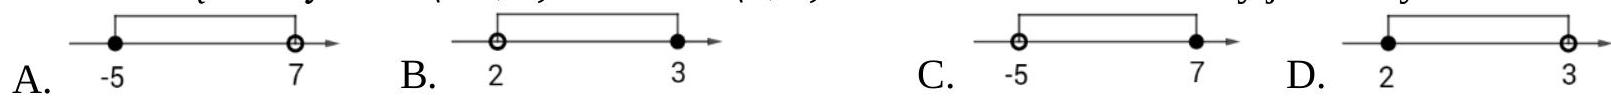
\includegraphics[max width=\textwidth, center]{2024_11_21_87037534e5fdc524263ag-02}

Zadanie 2. (1pkt)\\
Liczba ||4-7| - |13-5|| jest równa:\\
A. 29\\
B. 5\\
C. 7\\
D. 11

Zadanie 3. (1pkt)\\
Odwrotnością liczby \(2 \sqrt{2}-3\) jest liczba:\\
A. \(3-2 \sqrt{2}\)\\
B. \(2 \sqrt{2}+3\)\\
C. \(-3-2 \sqrt{2}\)\\
D. \(\frac{1}{2 \sqrt{2}+3}\)

Zadanie 4. (1pkt)\\
Liczba \(\sqrt[3]{9^{6} \cdot\left(\frac{1}{3}\right)^{9}: 27^{-1}}\) jest równa:\\
A. \(3^{0}\)\\
B. \(3^{2}\)\\
C. \(3^{6}\)\\
D. \(3^{8}\)

Zadanie 5. (1pkt)\\
Liczba \(-2 \log _{3} 6+3 \log _{3} 2\) jest równa:\\
A. \(\log _{3} \frac{2}{9}\)\\
B. -1\\
C. \(\log _{3} \frac{1}{18}\)\\
D. \(\log _{3} 288\)

Zadanie 6. (1pkt)\\
Liczba \(\sqrt{128}-0,5 \sqrt{32}\) jest równa:\\
A. \(\sqrt{112}\)\\
B. \(6 \sqrt{2}\)\\
C. \(\sqrt{8}\)\\
D. \(4 \sqrt{2}\)

\section*{Zadanie 7. (1pkt)}
Koszt uczestnictwa w obozie sportowym w 2018 r. wynosi 1620 zł. Wzrósł on w stosunku do kosztu z 2017 r. o 35\%. Koszt uczestnictwa w obozie w 2017 r. wynosił:\\
A. 1215 zt\\
B. 1053 zt\\
C. 1200 zt\\
D. \(567 \mathrm{zł}\)

\section*{Zadanie 8. (1pkt)}
Wartość wyrażenia \(\left(-1-x^{3}\right)\left(x^{3}-1\right)\) dla \(x=-\sqrt[3]{3}\) jest równa:\\
A. -8\\
B. 2\\
C. -4\\
D. -2

\section*{Zadanie 9. (1pkt)}
Do zbioru rozwiązań równania \(x(x+2)\left(x^{2}-1\right)=0\) nie należy liczba:\\
A. 0\\
B. 1\\
C. 2\\
D. -1

Zadanie 10. (1pkt)\\
Wartość wyrażenia \((4-\sqrt{3})^{2}-(4+\sqrt{3})^{2}\) wynosi:\\
A. -6\\
B. \(-4 \sqrt{3}\)\\
C. 6\\
D. \(-16 \sqrt{3}\)

Zadanie 11. (1pkt)\\
Marta oszacowała, że wyda na zakupy około 50 zł. W rzeczywistości zapłaciła 48 zł. Błąd względny, jaki popełniła szacując wartość zakupów wynosi:\\
A. \(\frac{1}{25}\)\\
B. \(\frac{1}{24}\)\\
C. 2\\
D. \(\frac{2}{25}\)

Zadanie 12. (1pkt)\\
Dany jest zbiór \(A=\left\{\frac{\pi}{2} ;-1 ; \sqrt{7 \frac{1}{9}} ; 0 ; 1,(3) ; \frac{1-\sqrt{3}}{4}\right\}\). Liczb wymiernych w zbiorze A jest:\\
A. pięć\\
B. dwie\\
C. trzy\\
D. cztery

Zadanie 13. (1pkt)\\
Układ równań \(\left\{\begin{array}{c}3 x-4 y=5 \\ -6 x+(a+3) y=10\end{array}\right.\) jest sprzeczny dla:\\
A. \(a=-11\)\\
B. \(a=5\)\\
C. \(a=3\)\\
D. \(a=-2\)

Zadanie 14. (1pkt)\\
Odcinek AB jest średnicą okręgu (rysunek).\\
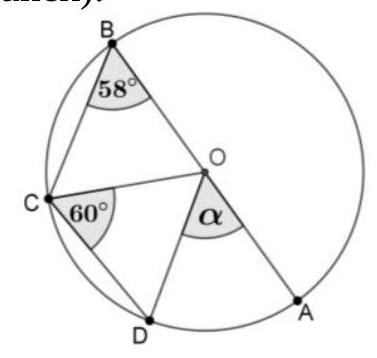
\includegraphics[max width=\textwidth, center]{2024_11_21_87037534e5fdc524263ag-04}

Miara kąta \(\alpha\) jest równa:\\
A. \(58^{\circ}\)\\
B. \(56^{\circ}\)\\
C. \(60^{\circ}\)\\
D. \(116^{\circ}\)

Zadanie 15. (1pkt)\\
Długości boków trójkąta nie mogą być równe:\\
A. \(3 ; 4 ; 4\)\\
B. \(3 ; 4 ; 5\)\\
C. \(3 ; 4 ; 2\)\\
D. \(3 ; 4 ; 8\)

Zadanie 16. (1pkt)\\
Dwa boki trójkąta prostokątnego mają długości 3 cm oraz 4 cm . Długość najkrótszego boku tego trójkąta wynosi:\\
A. 5 cm\\
B. \(\sqrt{7} \mathrm{~cm}\)\\
C. \(2,6 \mathrm{~cm}\)\\
D. \(\sqrt{5} \mathrm{~cm}\)

Zadanie 17. (1pkt)\\
Pole koła opisanego na trójkącie prostokątnym o bokach długości 10, 24, 26 jest równe:\\
A. \(144 \pi\)\\
B. \(25 \pi\)\\
C. \(169 \pi\)\\
D. \(26 \pi\)

Zadanie 18. (1pkt)\\
Trójkąty ABC oraz A'B'C' są podobne. Obwód trójkąta A'B'C' jest równy 12, a jego pole 6. Jeżeli pole trójkąta ABC jest równe \(13 \frac{1}{2}\), to jego obwód wynosi:\\
A. 18\\
B. \(6 \frac{3}{4}\)\\
C. 27\\
D. 9

Zadanie 19. (1pkt)\\
Na końcowym ramieniu kąta \(\alpha\) (rysunek) leży punkt \(\mathrm{P}=(-3 ; 4)\).\\
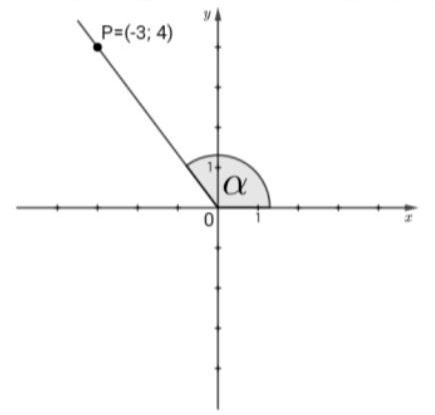
\includegraphics[max width=\textwidth, center]{2024_11_21_87037534e5fdc524263ag-06}

Wówczas:\\
A. \(\sin \alpha=-\frac{3}{5}\)\\
B. \(\cos \alpha=-\frac{4}{3}\)\\
C. \(\cos \alpha=-\frac{3}{5}\)\\
D. \(\operatorname{tg} \alpha=\frac{4}{3}\)

Zadanie 20. (1pkt)\\
Długość boku AC w trójkącie przedstawionym na poniższym rysunku jest równa:\\
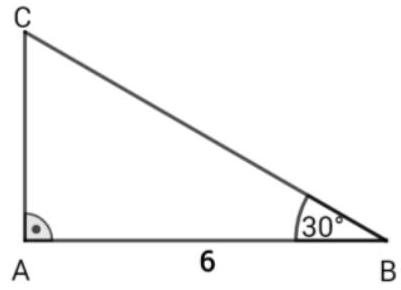
\includegraphics[max width=\textwidth, center]{2024_11_21_87037534e5fdc524263ag-06(1)}\\
A. 3\\
B. \(3 \sqrt{2}\)\\
C. \(6 \sqrt{3}\)\\
D. \(2 \sqrt{3}\)

Zadanie 21. (1pkt)\\
Wartość wyrażenia \(\cos 120^{\circ} \cdot \operatorname{tg} 120^{\circ}\) wynosi:\\
A. \(-\frac{\sqrt{3}}{2}\)\\
B. 1\\
C. \(\frac{1}{2}\)\\
D. \(\frac{\sqrt{3}}{2}\)

\section*{Zadanie 22. (1pkt)}
Długość okręgu wpisanego w trójkąt równoboczny wynosi \(6 \pi\). Długość boku tego trójkąta jest równa:\\
A. 9\\
B. \(6 \sqrt{3}\)\\
C. \(2 \sqrt{3}\)\\
D. 6

Zadanie 23. (1pkt)\\
Zbiór \(\boldsymbol{R} \backslash\{3\}\) jest dziedziną funkcji:\\
A. \(f(x)=\frac{x}{(x-3)^{2}}\)\\
B. \(f(x)=\frac{2}{x^{2}-9}\)\\
C. \(f(x)=\frac{x+3}{x^{2}-3}\)\\
D. \(f(x)=x-3\)

\section*{Zadanie 24. (1pkt)}
Do wykresu funkcji \(f(x)=2 \sqrt{3} x-4\) należy punkt o współrzędnych:\\
A. \((-4 ; 0)\)\\
B. \((\sqrt{3} ;-2)\)\\
C. \((-\sqrt{3} ;-10)\)\\
D. \((2 \sqrt{3} ; 2)\)

\section*{Zadanie 25. (1pkt)}
Wykres funkcji \(f(x)=(x-3)^{2}\) przesunięto równolegle o 2 jednostki w prawo. W wyniku tego przekształcenia otrzymano wykres funkcji:\\
A. \(g(x)=(x-5)^{2}\)\\
B. \(g(x)=(x-3)^{2}+2\)\\
C. \(g(x)=(x-1)^{2}\)\\
D. \(g(x)=(x-3)^{2}-2\)

\section*{ZADANIA OTWARTE}
Rozwiązania zadań o numerach od 26 do 34 należy zapisać w wyznaczonych miejscach pod treścią zadania.\\
Zadanie 26. (2 pkt)\\
Rozwiąż równanie \((x-3)(x+3)+5=(x-2)^{2}\).

\begin{center}
\begin{tabular}{|c|c|c|c|c|c|c|c|c|c|c|c|c|c|c|c|c|c|c|c|c|c|c|c|c|c|c|c|c|c|c|}
\hline
 &  &  &  &  &  &  &  &  &  &  &  &  &  &  &  &  &  &  &  &  &  &  &  &  &  &  &  &  &  &  \\
\hline
 &  &  &  &  &  &  &  &  &  &  &  &  &  &  &  &  &  &  &  &  &  &  &  &  &  &  &  &  &  &  \\
\hline
 &  &  &  &  &  &  &  &  &  &  &  &  &  &  &  &  &  &  &  &  &  &  &  &  &  &  &  &  &  &  \\
\hline
 &  &  &  &  &  &  &  &  &  &  &  &  &  &  &  &  &  &  &  &  &  &  &  &  &  &  &  &  &  &  \\
\hline
 &  &  &  &  &  &  &  &  &  &  &  &  &  &  &  &  &  &  &  &  &  &  &  &  &  &  &  &  &  &  \\
\hline
 &  &  &  &  &  &  &  &  &  &  &  &  &  &  &  &  &  &  &  &  &  &  &  &  &  &  &  &  &  &  \\
\hline
 &  &  &  &  &  &  &  &  &  &  &  &  &  &  &  &  &  &  &  &  &  &  &  &  &  &  &  &  &  &  \\
\hline
 &  &  &  &  &  &  &  &  &  &  &  &  &  &  &  &  &  &  &  &  &  &  &  &  &  &  &  &  &  &  \\
\hline
 &  &  &  &  &  &  &  &  &  &  &  &  &  &  &  &  &  &  &  &  &  &  &  &  &  &  &  &  &  &  \\
\hline
 &  &  &  &  &  &  &  &  &  &  &  &  &  &  &  &  &  &  &  &  &  &  &  &  &  &  &  &  &  &  \\
\hline
 &  &  &  &  &  &  &  &  &  &  &  &  &  &  &  &  &  &  &  &  &  &  &  &  &  &  &  &  &  &  \\
\hline
 &  &  &  &  &  &  &  &  &  &  &  &  &  &  &  &  &  &  &  &  &  &  &  &  &  &  &  &  &  &  \\
\hline
 &  &  &  &  &  &  &  &  &  &  &  &  &  &  &  &  &  &  &  &  &  &  &  &  &  &  &  &  &  &  \\
\hline
 &  &  &  &  &  &  &  &  &  &  &  &  &  &  &  &  &  &  &  &  &  &  &  &  &  &  &  &  &  &  \\
\hline
 &  &  &  &  &  &  &  &  &  &  &  &  &  &  &  &  &  &  &  &  &  &  &  &  &  &  &  &  &  &  \\
\hline
 &  &  &  &  &  &  &  &  &  &  &  &  &  &  &  &  &  &  &  &  &  &  &  &  &  &  &  &  &  &  \\
\hline
 &  &  &  &  &  &  &  &  &  &  &  &  &  &  &  &  &  &  &  &  &  &  &  &  &  &  &  &  &  &  \\
\hline
 &  &  &  &  &  &  &  &  &  &  &  &  &  &  &  &  &  &  &  &  &  &  &  &  &  &  &  &  &  &  \\
\hline
 &  &  &  &  &  &  &  &  &  &  &  &  &  &  &  &  &  &  &  &  &  &  &  &  &  &  &  & 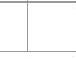
\includegraphics[max width=\textwidth]{2024_11_21_87037534e5fdc524263ag-08}
 &  &  \\
\hline
\end{tabular}
\end{center}

Zadanie 27. (2 pkt)\\
Wykaż, że jeżeli \(a+b=6\), to \(a^{2}+b^{2} \geq 18\).

\begin{center}
\begin{tabular}{|c|c|c|c|c|c|c|c|c|c|c|c|c|c|c|c|c|c|c|c|c|c|c|c|c|c|c|c|c|c|c|c|}
\hline
 &  &  &  &  &  &  &  &  &  &  &  &  &  &  &  &  &  &  &  &  &  &  &  &  &  &  &  &  &  &  &  \\
\hline
 &  &  &  &  &  &  &  &  &  &  &  &  &  &  &  &  &  &  &  &  &  &  &  &  &  &  &  &  &  &  &  \\
\hline
 &  &  &  &  &  &  &  &  &  &  &  &  &  &  &  &  &  &  &  &  &  &  &  &  &  &  &  &  &  &  &  \\
\hline
 &  &  &  &  &  &  &  &  &  &  &  &  &  &  &  &  &  &  &  &  &  &  &  &  &  &  &  &  &  &  &  \\
\hline
 &  &  &  &  &  &  &  &  &  &  &  &  &  &  &  &  &  &  &  &  &  &  &  &  &  &  &  &  &  &  &  \\
\hline
 &  &  &  &  &  &  &  &  &  &  &  &  &  &  &  &  &  &  &  &  &  &  &  &  &  &  &  &  &  &  &  \\
\hline
 &  &  &  &  &  &  &  &  &  &  &  &  &  &  &  &  &  &  &  &  &  &  &  &  &  &  &  &  &  &  &  \\
\hline
 &  &  &  &  &  &  &  &  &  &  &  &  &  &  &  &  &  &  &  &  &  &  &  &  &  &  &  &  &  &  &  \\
\hline
 &  &  &  &  &  &  &  &  &  &  &  &  &  &  &  &  &  &  &  &  &  &  &  &  &  &  &  &  &  &  &  \\
\hline
 &  &  &  &  &  &  &  &  &  &  &  &  &  &  &  &  &  &  &  &  &  &  &  &  &  &  &  &  &  &  &  \\
\hline
 &  &  &  &  &  &  &  &  &  &  &  &  &  &  &  &  &  &  &  &  &  &  &  &  &  &  &  &  &  &  &  \\
\hline
 &  &  &  &  &  &  &  &  &  &  &  &  &  &  &  &  &  &  &  &  &  &  &  &  &  &  &  &  &  &  &  \\
\hline
 &  &  &  &  &  &  &  &  &  &  &  &  &  &  &  &  &  &  &  &  &  &  &  &  &  &  &  &  &  &  &  \\
\hline
 &  &  &  &  &  &  &  &  &  &  &  &  &  &  &  &  &  &  &  &  &  &  &  &  &  &  &  &  &  &  &  \\
\hline
 &  &  &  &  &  &  &  &  &  &  &  &  &  &  &  &  &  &  &  &  &  &  &  &  &  &  &  &  &  &  &  \\
\hline
 &  &  &  &  &  &  &  &  &  &  &  &  &  &  &  &  &  &  &  &  &  &  &  &  &  &  &  &  &  &  &  \\
\hline
 &  &  &  &  &  &  &  &  &  &  &  &  &  &  &  &  &  &  &  &  &  &  &  &  &  &  &  &  &  &  &  \\
\hline
 &  &  &  &  &  &  &  &  &  &  &  &  &  &  &  &  &  &  &  &  &  &  &  &  &  &  &  &  &  &  &  \\
\hline
 &  &  &  &  &  &  &  &  &  &  &  &  &  &  &  &  &  &  &  &  &  &  &  &  &  &  &  &  &  &  &  \\
\hline
 &  &  &  &  &  &  &  &  &  &  &  &  &  &  &  &  &  &  &  &  &  &  &  &  &  &  &  &  &  &  &  \\
\hline
\end{tabular}
\end{center}

Zadanie 28. (2 pkt)\\
Kąt \(\alpha\) jest ostry i \(\sin \alpha=\frac{\sqrt{7}}{4}\). Oblicz wartość wyrażenia: \(\cos ^{3} \alpha-4 \sin ^{2} \alpha\).

\begin{center}
\begin{tabular}{|c|c|c|c|c|c|c|c|c|c|c|c|c|c|c|c|c|c|c|c|c|c|c|c|c|c|c|c|c|c|c|}
\hline
 &  &  &  &  &  &  &  &  &  &  &  &  &  &  &  &  &  &  &  &  &  &  &  &  &  &  &  &  &  &  \\
\hline
 &  &  &  &  &  &  &  &  &  &  &  &  &  &  &  &  &  &  &  &  &  &  &  &  &  &  &  &  &  &  \\
\hline
 &  &  &  &  &  &  &  &  &  &  &  &  &  &  &  &  &  &  &  &  &  &  &  &  &  &  &  &  &  &  \\
\hline
 &  &  &  &  &  &  &  &  &  &  &  &  &  &  &  &  &  &  &  &  &  &  &  &  &  &  &  &  &  &  \\
\hline
 &  &  &  &  &  &  &  &  &  &  &  &  &  &  &  &  &  &  &  &  &  &  &  &  &  &  &  &  &  &  \\
\hline
 &  &  &  &  &  &  &  &  &  &  &  &  &  &  &  &  &  &  &  &  &  &  &  &  &  &  &  &  &  &  \\
\hline
 &  &  &  &  &  &  &  &  &  &  &  &  &  &  &  &  &  &  &  &  &  &  &  &  &  &  &  &  &  &  \\
\hline
 &  &  &  &  &  &  &  &  &  &  &  &  &  &  &  &  &  &  &  &  &  &  &  &  &  &  &  &  &  &  \\
\hline
 &  &  &  &  &  &  &  &  &  &  &  &  &  &  &  &  &  &  &  &  &  &  &  &  &  &  &  &  &  &  \\
\hline
 &  &  &  &  &  &  &  &  &  &  &  &  &  &  &  &  &  &  &  &  &  &  &  &  &  &  &  &  &  &  \\
\hline
 &  &  &  &  &  &  &  &  &  &  &  &  &  &  &  &  &  &  &  &  &  &  &  &  &  &  &  &  &  &  \\
\hline
 &  &  &  &  &  &  &  &  &  &  &  &  &  &  &  &  &  &  &  &  &  &  &  &  &  &  &  &  &  &  \\
\hline
 &  &  &  &  &  &  &  &  &  &  &  &  &  &  &  &  &  &  &  &  &  &  &  &  &  &  &  &  &  &  \\
\hline
 &  &  &  &  &  &  &  &  &  &  &  &  &  &  &  &  &  &  &  &  &  &  &  &  &  &  &  &  &  &  \\
\hline
 &  &  &  &  &  &  &  &  &  &  &  &  &  &  &  &  &  &  &  &  &  &  &  &  &  &  &  &  &  &  \\
\hline
 &  &  &  &  &  &  &  &  &  &  &  &  &  &  &  &  &  &  &  &  &  &  &  &  &  &  &  &  &  &  \\
\hline
 &  &  &  &  &  &  &  &  &  &  &  &  &  &  &  &  &  &  &  &  &  &  &  &  &  &  &  &  &  &  \\
\hline
 &  &  &  &  &  &  &  &  &  &  &  &  &  &  &  &  &  &  &  &  &  &  &  &  &  &  &  &  &  &  \\
\hline
 &  &  &  &  &  &  &  &  &  &  &  &  &  &  &  &  &  &  &  &  &  &  &  &  &  &  &  & \( 0 \) &  &  \\
\hline
\end{tabular}
\end{center}

Zadanie 29. (2 pkt)\\
Trójkąt ABC jest prostokątny. Z punktu M należącego do przeciwprostokątnej BC poprowadzono odcinki MD oraz MS prostopadłe odpowiednio do przyprostokątnych AC ora AB (rysunek).\\
Wykaż, że \(\frac{|D M|}{|A B|}+\frac{|M S|}{|A C|}=1\).\\

\includegraphics[max width=\textwidth, center]{2024_11_21_87037534e5fdc524263ag-09}

Zadanie 30. (2 pkt)\\
W trójkącie ABC dane są: \(|A C|=|B C|=8\) oraz \(|\Varangle A C B|=45^{\circ}\). Oblicz długość wysokości tego trójkąta poprowadzonej z wierzchołka A.

\begin{center}
\begin{tabular}{|c|c|c|c|c|c|c|c|c|c|c|c|c|c|c|c|c|c|c|c|c|c|c|c|c|c|c|c|c|c|c|c|}
\hline
 &  &  &  &  &  &  &  &  &  &  &  &  &  &  &  &  &  &  &  &  &  &  &  &  &  &  &  &  &  &  &  \\
\hline
 &  &  &  &  &  &  &  &  &  &  &  &  &  &  &  &  &  &  &  &  &  &  &  &  &  &  &  &  &  &  &  \\
\hline
 &  &  &  &  &  &  &  &  &  &  &  &  &  &  &  &  &  &  &  &  &  &  &  &  &  &  &  &  &  &  &  \\
\hline
 &  &  &  &  &  &  &  &  &  &  &  &  &  &  &  &  &  &  &  &  &  &  &  &  &  &  &  &  &  &  &  \\
\hline
 &  &  &  &  &  &  &  &  &  &  &  &  &  &  &  &  &  &  &  &  &  &  &  &  &  &  &  &  &  &  &  \\
\hline
 &  &  &  &  &  &  &  &  &  &  &  &  &  &  &  &  &  &  &  &  &  &  &  &  &  &  &  &  &  &  &  \\
\hline
 &  &  &  &  &  &  &  &  &  &  &  &  &  &  &  &  &  &  &  &  &  &  &  &  &  &  &  &  &  &  &  \\
\hline
 &  &  &  &  &  &  &  &  &  &  &  &  &  &  &  &  &  &  &  &  &  &  &  &  &  &  &  &  &  &  &  \\
\hline
 &  &  &  &  &  &  &  &  &  &  &  &  &  &  &  &  &  &  &  &  &  &  &  &  &  &  &  &  &  &  &  \\
\hline
 &  &  &  &  &  &  &  &  &  &  &  &  &  &  &  &  &  &  &  &  &  &  &  &  &  &  &  &  &  &  &  \\
\hline
 &  &  &  &  &  &  &  &  &  &  &  &  &  &  &  &  &  &  &  &  &  &  &  &  &  &  &  &  &  &  &  \\
\hline
 &  &  &  &  &  &  &  &  &  &  &  &  &  &  &  &  &  &  &  &  &  &  &  &  &  &  &  &  &  &  &  \\
\hline
 &  &  &  &  &  &  &  &  &  &  &  &  &  &  &  &  &  &  &  &  &  &  &  &  &  &  &  &  &  &  &  \\
\hline
 &  &  &  &  &  &  &  &  &  &  &  &  &  &  &  &  &  &  &  &  &  &  &  &  &  &  &  &  &  &  &  \\
\hline
 &  &  &  &  &  &  &  &  &  &  &  &  &  &  &  &  &  &  &  &  &  &  &  &  &  &  &  &  &  &  &  \\
\hline
 &  &  &  &  &  &  &  &  &  &  &  &  &  &  &  &  &  &  &  &  &  &  &  &  &  &  &  &  &  &  &  \\
\hline
 &  &  &  &  &  &  &  &  &  &  &  &  &  &  &  &  &  &  &  &  &  &  &  &  &  &  &  &  &  &  &  \\
\hline
 &  &  &  &  &  &  &  &  &  &  &  &  &  &  &  &  &  &  &  &  &  &  &  &  &  &  &  &  &  &  &  \\
\hline
 &  &  &  &  &  &  &  &  &  &  &  &  &  &  &  &  &  &  &  &  &  &  &  &  &  &  &  &  &  &  &  \\
\hline
 &  &  &  &  &  &  &  &  &  &  &  &  &  &  &  &  &  &  &  &  &  &  &  &  &  &  &  &  &  &  &  \\
\hline
 &  &  &  &  &  &  &  &  &  &  &  &  &  &  &  &  &  &  &  &  &  &  &  &  &  &  &  &  &  &  &  \\
\hline
\end{tabular}
\end{center}

Zadanie 31. (2 pkt)\\
Odcinki \(A B\) oraz \(B C\) (rysunek) są równej długości. Kąt ABC ma miarę o \(124^{\circ}\) mniejszą od miary kąta do niego przyległego. Oblicz miarę kąta ACD.\\

\includegraphics[max width=\textwidth, center]{2024_11_21_87037534e5fdc524263ag-10}

Zadanie 32. (5 pkt)\\
Poniżej przedstawiony jest wykres funkcji \(y=f(x)\). Na podstawie tego wykresu podaj:\\
a) dziedzinę funkcji \(f\),\\
b) zbiór wartości funkcji \(f\),\\
c) maksymalne przedziały, w których funkcja \(f\) jest malejąca,\\
d) miejsca zerowe funkcji \(f\),\\
e) zbiór argumentów, dla których funkcja f przyjmuje wartości nieujemne.\\
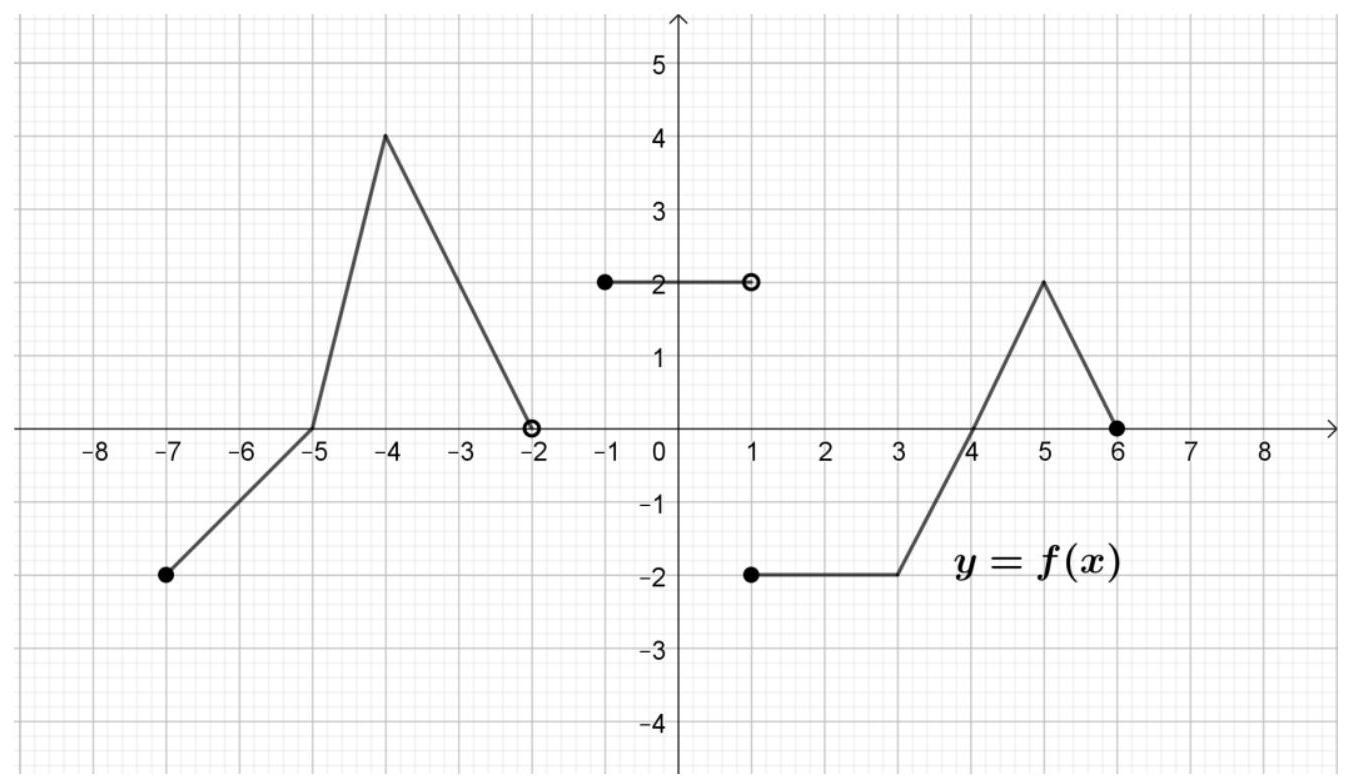
\includegraphics[max width=\textwidth, center]{2024_11_21_87037534e5fdc524263ag-11}\\

\includegraphics[max width=\textwidth, center]{2024_11_21_87037534e5fdc524263ag-11(1)}

Zadanie 33. (4 pkt)\\
Karol zarabiał miesięcznie 4200 zł, a Jan 3800 zł. Obaj otrzymali w swoich firmach podwyżki.\\
Podwyżka otrzymana przez Jana była o 3 punkty procentowe wyższa niż podwyżka otrzymana przez Karola. Po podwyżce obaj panowie zarabiają łącznie 9074 zł. Ile zarabia każdy z panów po podwyżce? Zapisz wszystkie obliczenia.\\

\includegraphics[max width=\textwidth, center]{2024_11_21_87037534e5fdc524263ag-12}

Zadanie 34. (4 pkt)\\
Wyznacz wszystkie liczby pierwsze, które należą do zbioru \(A \backslash B\), gdzie \(A\) jest zbiorem rozwiązań nierówności:

\[
\left(\log _{6} 18-\log _{6} 3\right)+2 x \geq-2-x
\]

a \(B\) jest zbiorem rozwiązań nierówności:

\[
1-\frac{x-2}{3}<-2
\]

\begin{center}
\begin{tabular}{|c|c|c|c|c|c|c|c|c|c|c|c|c|c|c|c|c|c|c|c|c|c|c|c|c|}
\hline
 &  &  &  &  &  &  &  &  &  &  &  &  &  &  &  &  &  &  &  &  &  &  &  &  \\
\hline
 &  &  &  &  &  &  &  &  &  &  &  &  &  &  &  &  &  &  &  &  &  &  &  &  \\
\hline
 &  &  &  &  &  &  &  &  &  &  &  &  &  &  &  &  &  &  &  &  &  &  &  &  \\
\hline
 &  &  &  &  &  &  &  &  &  &  &  &  &  &  &  &  &  &  &  &  &  &  &  &  \\
\hline
 &  &  &  &  &  &  &  &  &  &  &  &  &  &  &  &  &  &  &  &  &  &  &  &  \\
\hline
 &  &  &  &  &  &  &  &  &  &  &  &  &  &  &  &  &  &  &  &  &  &  &  &  \\
\hline
 &  &  &  &  &  &  &  &  &  &  &  &  &  &  &  &  &  &  &  &  &  &  &  &  \\
\hline
 &  &  &  &  &  &  &  &  &  &  &  &  &  &  &  &  &  &  &  &  &  &  &  &  \\
\hline
 &  &  &  &  &  &  &  &  &  &  &  &  &  &  &  &  &  &  &  &  &  &  &  &  \\
\hline
 &  &  &  &  &  &  &  &  &  &  &  &  &  &  &  &  &  &  &  &  &  &  &  &  \\
\hline
 &  &  &  &  &  &  &  &  &  &  &  &  &  &  &  &  &  &  &  &  &  &  &  &  \\
\hline
 &  &  &  &  &  &  &  &  &  &  &  &  &  &  &  &  &  &  &  &  &  &  &  &  \\
\hline
 &  &  &  &  &  &  &  &  &  &  &  &  &  &  &  &  &  &  &  &  &  &  &  &  \\
\hline
 &  &  &  &  &  &  &  &  &  &  &  &  &  &  &  &  &  &  &  &  &  &  &  &  \\
\hline
 &  &  &  &  &  &  &  &  &  &  &  &  &  &  &  &  &  &  &  &  &  &  &  &  \\
\hline
 &  &  &  &  &  &  &  &  &  &  &  &  &  &  &  &  &  &  &  &  &  &  &  &  \\
\hline
 &  &  &  &  &  &  &  &  &  &  &  &  &  &  &  &  &  &  &  &  &  &  &  &  \\
\hline
 &  &  &  &  &  &  &  &  &  &  &  &  &  &  &  &  &  &  &  &  &  &  &  &  \\
\hline
 &  &  &  &  &  &  &  &  &  &  &  &  &  &  &  &  &  &  &  &  &  &  &  &  \\
\hline
 &  &  &  &  &  &  &  &  &  &  &  &  &  &  &  &  &  &  &  &  &  &  &  &  \\
\hline
 &  &  &  &  &  &  &  &  &  &  &  &  &  &  &  &  &  &  &  &  &  &  &  &  \\
\hline
 &  &  &  &  &  &  &  &  &  &  &  &  &  &  &  &  &  &  &  &  &  &  &  &  \\
\hline
 &  &  &  &  &  &  &  &  &  &  &  &  &  &  &  &  &  &  &  &  &  &  &  &  \\
\hline
 &  &  &  &  &  &  &  &  &  &  &  &  &  &  &  &  &  &  &  &  &  &  &  &  \\
\hline
 &  &  &  &  &  &  &  &  &  &  &  &  &  &  &  &  &  &  &  &  &  &  &  &  \\
\hline
 &  &  &  &  &  &  &  &  &  &  &  &  &  &  &  &  &  &  &  &  &  &  &  &  \\
\hline
 &  &  &  &  &  &  &  &  &  &  &  &  &  &  &  &  &  &  &  &  &  &  &  &  \\
\hline
 &  &  &  &  &  &  &  &  &  &  &  &  &  &  &  &  &  &  &  &  &  &  &  &  \\
\hline
 &  &  &  &  &  &  &  &  &  &  &  &  &  &  &  &  &  &  &  &  &  &  &  &  \\
\hline
 &  &  &  &  &  &  &  &  &  &  &  &  &  &  &  &  &  &  &  &  &  &  &  &  \\
\hline
 &  &  &  &  &  &  &  &  &  &  &  &  &  &  &  &  &  &  &  &  &  &  &  &  \\
\hline
 &  &  &  &  &  &  &  &  &  &  &  &  &  &  &  &  &  &  &  &  &  &  &  &  \\
\hline
 &  &  &  &  &  &  &  &  &  &  &  &  &  &  &  &  &  &  &  &  &  &  &  &  \\
\hline
 &  &  &  &  &  &  &  &  &  &  &  &  &  &  &  &  &  &  &  &  &  &  &  &  \\
\hline
 &  &  &  &  &  &  &  &  &  &  &  &  &  &  &  &  &  &  &  &  &  &  &  &  \\
\hline
 &  &  &  &  &  &  &  &  &  &  &  &  &  &  &  &  &  &  &  &  &  &  &  &  \\
\hline
 &  &  &  &  &  &  &  &  &  &  &  &  &  &  &  &  &  &  &  &  &  &  &  &  \\
\hline
 &  &  &  &  &  &  &  &  &  &  &  &  &  &  &  &  &  &  &  &  &  &  &  &  \\
\hline
 &  &  &  &  &  &  &  &  &  &  &  &  &  &  &  &  &  &  &  &  &  &  &  &  \\
\hline
 &  &  &  &  &  &  &  &  &  &  &  &  &  &  &  &  &  &  &  &  &  &  &  &  \\
\hline
 &  &  &  &  &  &  &  &  &  &  &  &  &  &  &  &  &  &  &  &  &  &  &  &  \\
\hline
 &  &  &  &  &  &  &  &  &  &  &  &  &  &  &  &  &  &  &  &  &  &  &  &  \\
\hline
\end{tabular}
\end{center}

\begin{center}
\begin{tabular}{|c|c|c|c|c|c|c|c|c|c|c|c|c|c|c|c|c|c|c|c|c|c|c|c|c|}
\hline
 &  &  &  &  &  &  &  &  &  &  &  &  &  &  &  &  &  &  &  &  &  &  &  &  \\
\hline
 &  &  &  &  &  &  &  &  &  &  &  &  &  &  &  &  &  &  &  &  &  &  &  &  \\
\hline
 &  &  &  &  &  &  &  &  &  &  &  &  &  &  &  &  &  &  &  &  &  &  &  &  \\
\hline
 &  &  &  &  &  &  &  &  &  &  &  &  &  &  &  &  &  &  &  &  &  &  &  &  \\
\hline
 &  &  &  &  &  &  &  &  &  &  &  &  &  &  &  &  &  &  &  &  &  &  &  &  \\
\hline
 &  &  &  &  &  &  &  &  &  &  &  &  &  &  &  &  &  &  &  &  &  &  &  &  \\
\hline
 &  &  &  &  &  &  &  &  &  &  &  &  &  &  &  &  &  &  &  &  &  &  &  &  \\
\hline
 &  &  &  &  &  &  &  &  &  &  &  &  &  &  &  &  &  &  &  &  &  &  &  &  \\
\hline
 &  &  &  &  &  &  &  &  &  &  &  &  &  &  &  &  &  &  &  &  &  &  &  &  \\
\hline
 &  &  &  &  &  &  &  &  &  &  &  &  &  &  &  &  &  &  &  &  &  &  &  &  \\
\hline
 &  &  &  &  &  &  &  &  &  &  &  &  &  &  &  &  &  &  &  &  &  &  &  &  \\
\hline
 &  &  &  &  &  &  &  &  &  &  &  &  &  &  &  &  &  &  &  &  &  &  &  &  \\
\hline
 &  &  &  &  &  &  &  &  &  &  &  &  &  &  &  &  &  &  &  &  &  &  &  &  \\
\hline
 &  &  &  &  &  &  &  &  &  &  &  &  &  &  &  &  &  &  &  &  &  &  &  &  \\
\hline
 &  &  &  &  &  &  &  &  &  &  &  &  &  &  &  &  &  &  &  &  &  &  &  &  \\
\hline
 &  &  &  &  &  &  &  &  &  &  &  &  &  &  &  &  &  &  &  &  &  &  &  &  \\
\hline
 &  &  &  &  &  &  &  &  &  &  &  &  &  &  &  &  &  &  &  &  &  &  &  &  \\
\hline
 &  &  &  &  &  &  &  &  &  &  &  &  &  &  &  &  &  &  &  &  &  &  &  &  \\
\hline
 &  &  &  &  &  &  &  &  &  &  &  &  &  &  &  &  &  &  &  &  &  &  &  &  \\
\hline
 &  &  &  &  &  &  &  &  &  &  &  &  &  &  &  &  &  &  &  &  &  &  &  &  \\
\hline
 &  &  &  &  &  &  &  &  &  &  &  &  &  &  &  &  &  &  &  &  &  &  &  &  \\
\hline
 &  &  &  &  &  &  &  &  &  &  &  &  &  &  &  &  &  &  &  &  &  &  &  &  \\
\hline
 &  &  &  &  &  &  &  &  &  &  &  &  &  &  &  &  &  &  &  &  &  &  &  &  \\
\hline
 &  &  &  &  &  &  &  &  &  &  &  &  &  &  &  &  &  &  &  &  &  &  &  &  \\
\hline
 &  &  &  &  &  &  &  &  &  &  &  &  &  &  &  &  &  &  &  &  &  &  &  &  \\
\hline
 &  &  &  &  &  &  &  &  &  &  &  &  &  &  &  &  &  &  &  &  &  &  &  &  \\
\hline
 &  &  &  &  &  &  &  &  &  &  &  &  &  &  &  &  &  &  &  &  &  &  &  &  \\
\hline
 &  &  &  &  &  &  &  &  &  &  &  &  &  &  &  &  &  &  &  &  &  &  &  &  \\
\hline
 &  &  &  &  &  &  &  &  &  &  &  &  &  &  &  &  &  &  &  &  &  &  &  &  \\
\hline
 & 到 &  &  &  &  &  &  &  &  &  &  &  &  &  &  &  &  &  &  &  &  &  &  &  \\
\hline
 &  &  &  &  &  &  &  &  &  &  &  &  &  &  &  &  &  &  &  &  &  &  &  &  \\
\hline
 &  &  &  &  &  &  &  &  &  &  &  &  &  &  &  &  &  &  &  &  &  &  &  &  \\
\hline
 &  &  &  &  &  &  &  &  &  &  &  &  &  &  &  &  &  &  &  &  &  &  &  &  \\
\hline
 &  &  &  &  &  &  &  &  &  &  &  &  &  &  &  &  &  &  &  &  &  &  &  &  \\
\hline
 &  &  &  &  &  &  &  &  &  &  &  &  &  &  &  &  &  &  &  &  &  &  &  &  \\
\hline
 &  &  &  &  &  &  &  &  &  &  &  &  &  &  &  &  &  &  &  &  &  &  &  &  \\
\hline
 &  &  &  &  &  &  &  &  &  &  &  &  &  &  &  &  &  &  &  &  &  &  &  &  \\
\hline
 &  &  &  &  &  &  &  &  &  &  &  &  &  &  &  &  &  &  &  &  &  &  &  &  \\
\hline
 &  &  &  &  &  &  &  &  &  &  &  &  &  &  &  &  &  &  &  &  &  &  &  &  \\
\hline
 &  &  &  &  &  &  &  &  &  &  &  &  &  &  &  &  &  &  &  &  &  &  &  &  \\
\hline
 &  &  &  &  &  &  &  &  &  &  &  &  &  &  &  &  &  &  &  &  &  &  &  &  \\
\hline
 &  &  &  &  &  &  &  &  &  &  &  &  &  &  &  &  &  &  &  &  &  &  &  &  \\
\hline
 &  &  &  &  &  &  &  &  &  &  &  &  &  &  &  &  &  &  &  &  &  &  &  &  \\
\hline
 &  &  &  &  &  &  &  &  &  &  &  &  &  &  &  &  &  &  &  &  &  &  &  &  \\
\hline
 &  &  &  &  &  &  &  &  &  &  &  &  &  &  &  &  &  &  &  &  &  &  &  &  \\
\hline
 &  &  &  &  &  &  &  &  &  &  &  &  &  &  &  &  &  &  &  &  &  &  &  &  \\
\hline
 &  &  &  &  &  &  &  &  &  &  &  &  &  &  &  &  &  &  &  &  &  &  &  &  \\
\hline
 &  &  &  &  &  &  &  &  &  &  &  &  &  &  &  &  &  &  &  &  &  &  &  &  \\
\hline
 &  &  &  &  &  &  &  &  &  &  &  &  &  &  &  &  &  &  &  &  &  &  &  &  \\
\hline
\end{tabular}
\end{center}

\begin{center}
\begin{tabular}{|c|c|c|c|c|c|c|c|c|c|c|c|c|}
\hline
\multicolumn{5}{|c|}{WYPELNIA PISZACY} & \multicolumn{7}{|r|}{WYPELNIA SPRAWDZAJACY} &  \\
\hline
\( \underset{\text { zadania }}{\mathrm{Nr}} \) & A & B & C & D & \multicolumn{2}{|r|}{\multirow[b]{2}{*}{
\includegraphics[max width=\textwidth]{2024_11_21_87037534e5fdc524263ag-16}
}} & \multirow[b]{2}{*}{X} & \multirow[b]{2}{*}{0} & \multicolumn{2}{|c|}{\multirow[b]{2}{*}{1}} & \multirow[b]{2}{*}{2} &  \\
\hline
1. & \(\square\) & \(\square\) & \(\square\) & \(\square\) &  &  &  &  &  &  &  &  \\
\hline
2. & \(\square\) & \(\square\) & \(\square\) & \(\square\) &  & 26. & \(\square\) & \(\square\) &  &  & \(\square\) &  \\
\hline
3. & \(\square\) & \(\square\) & \(\square\) & \(\square\) &  & 27. & \(\square\) & \(\square\) &  &  & \(\square\) &  \\
\hline
4. & \(\square\) & \(\square\) & \(\square\) & \(\square\) &  & 28. & 口 & \(\square\) &  &  & \(\square\) &  \\
\hline
5. & \(\square\) & \(\square\) & \(\square\) & \(\square\) &  & 29. & \(\square\) & \(\square\) &  &  & \(\square\) &  \\
\hline
6. & \(\square\) & \(\square\) & \(\square\) & \(\square\) &  & 30. & \(\square\) & \(\square\) &  &  & \(\square\) &  \\
\hline
7. & \(\square\) & \(\square\) & \(\square\) & \(\square\) &  & \multirow[t]{2}{*}{31.} & \(\square\) & \(\square\) & \multicolumn{2}{|c|}{\multirow[t]{2}{*}{\(\square\)}} & \multirow[t]{2}{*}{\(\square\)} &  \\
\hline
8. & \(\square\) & \(\square\) & \(\square\) & \(\square\) &  &  &  &  &  &  &  &  \\
\hline
9. & \(\square\) & \(\square\) & \(\square\) & \(\square\) &  &  &  &  &  &  &  &  \\
\hline
10. & \(\square\) & \(\square\) & \(\square\) & \(\square\) & \multirow[t]{2}{*}{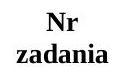
\includegraphics[max width=\textwidth]{2024_11_21_87037534e5fdc524263ag-16(2)}
} & \multirow[t]{2}{*}{X} & \multirow[t]{2}{*}{0} & \multirow[t]{2}{*}{1} & \multirow[t]{2}{*}{2} & \multirow[t]{2}{*}{3} & \multirow[t]{2}{*}{4} & \multirow[t]{2}{*}{5} \\
\hline
11. & \(\square\) & \(\square\) & \(\square\) & \(\square\) &  &  &  &  &  &  &  &  \\
\hline
12. & \(\square\) & \(\square\) & \(\square\) & \(\square\) & 32. & \(\square\) & \(\square\) & \(\square\) & \(\square\) & \(\square\) & \(\square\) & \(\square\) \\
\hline
13. & \(\square\) & \(\square\) & \(\square\) & \(\square\) & 33. & \(\square\) & \(\square\) & \(\square\) & 口 & ㅁ & \(\square\) &  \\
\hline
14. & \(\square\) & \(\square\) & \(\square\) & \(\square\) & 34. & \(\square\) & \(\square\) & \(\square\) & \(\square\) & ■ & \(\square\) &  \\
\hline
15. & \(\square\) & \(\square\) & \(\square\) & \(\square\) &  &  &  &  &  &  &  &  \\
\hline
16. & \(\square\) & \(\square\) & \(\square\) & \(\square\) &  &  &  &  &  &  &  &  \\
\hline
17. & \(\square\) & \(\square\) & \(\square\) & \(\square\) &  &  & \multicolumn{4}{|r|}{\multirow[t]{2}{*}{Suma punktów zadania otwarte}} &  &  \\
\hline
18. & \(\square\) & \(\square\) & \(\square\) & \(\square\) &  &  &  &  &  &  &  &  \\
\hline
19. & \(\square\) & \(\square\) & \(\square\) & \(\square\) &  &  &  &  &  &  &  &  \\
\hline
20. & \(\square\) & \(\square\) & \(\square\) & \(\square\) &  &  &  &  &  &  &  &  \\
\hline
21. & \(\square\) & \(\square\) & \(\square\) & \(\square\) &  &  &  &  &  &  &  &  \\
\hline
22. & \(\square\) & \(\square\) & \(\square\) & \(\square\) &  &  &  &  &  &  &  &  \\
\hline
23. & \(\square\) & \(\square\) & \(\square\) & \(\square\) &  &  &  &  &  &  &  &  \\
\hline
24. & \(\square\) & \(\square\) & \(\square\) & \(\square\) &  &  &  &  &  &  &  &  \\
\hline
25. & \(\square\) & \(\square\) & \(\square\) & \(\square\) &  &  &  &  &  &  &  &  \\
\hline
 &  & \begin{tabular}{l}
Sum \\
zadan \\
\end{tabular} & zun &  &  &  &  &  &  &  &  &  \\
\hline
 &  &  &  &  &  &  &  & \begin{tabular}{l}
Suma \\
a \\
\end{tabular} & 
\includegraphics[max width=\textwidth]{2024_11_21_87037534e5fdc524263ag-16(1)}
 &  &  &  \\
\hline
\end{tabular}
\end{center}


\end{document}